\documentclass[journal,12pt,twocolumn]{IEEEtran}
%
\usepackage{setspace}
\usepackage{gensymb}
%\doublespacing
\singlespacing

%\usepackage{graphicx}
%\usepackage{amssymb}
%\usepackage{relsize}
\usepackage[cmex10]{amsmath}
%\usepackage{amsthm}
%\interdisplaylinepenalty=2500
%\savesymbol{iint}
%\usepackage{txfonts}
%\restoresymbol{TXF}{iint}
%\usepackage{wasysym}
\usepackage{amsthm}
%\usepackage{iithtlc}
\usepackage{mathrsfs}
\usepackage{txfonts}
\usepackage{stfloats}
\usepackage{bm}
\usepackage{cite}
\usepackage{cases}
\usepackage{subfig}
%\usepackage{xtab}
\usepackage{longtable}
\usepackage{multirow}
%\usepackage{algorithm}
%\usepackage{algpseudocode}
\usepackage{enumitem}
\usepackage{mathtools}
\usepackage{steinmetz}
\usepackage{tikz}
\usepackage[american]{circuitikz}
\usepackage{verbatim}
\usepackage{tfrupee}
\usepackage[breaklinks=true]{hyperref}
%\usepackage{stmaryrd}
\usepackage{tkz-euclide} % loads  TikZ and tkz-base
\usetkzobj{all}
\usetikzlibrary{decorations.markings}
\usetikzlibrary{shapes.geometric}
\newif\iflabrev
\usepackage{listings}
    \usepackage{color}                                            %%
    \usepackage{array}                                            %%
    \usepackage{longtable}                                        %%
    \usepackage{calc}                                             %%
    \usepackage{multirow}                                         %%
    \usepackage{hhline}                                           %%
    \usepackage{ifthen}                                           %%
  %optionally (for landscape tables embedded in another document): %%
    \usepackage{lscape}     
\usepackage{multicol}
\usepackage{chngcntr}
%\usepackage{enumerate}

%\usepackage{wasysym}
%\newcounter{MYtempeqncnt}
\DeclareMathOperator*{\Res}{Res}
%\renewcommand{\baselinestretch}{2}
\renewcommand\thesection{\arabic{section}}
\renewcommand\thesubsection{\thesection.\arabic{subsection}}
\renewcommand\thesubsubsection{\thesubsection.\arabic{subsubsection}}

\renewcommand\thesectiondis{\arabic{section}}
\renewcommand\thesubsectiondis{\thesectiondis.\arabic{subsection}}
\renewcommand\thesubsubsectiondis{\thesubsectiondis.\arabic{subsubsection}}

% correct bad hyphenation here
\hyphenation{op-tical net-works semi-conduc-tor}
\def\inputGnumericTable{}                                 %%

\lstset{
%language=C,
frame=single, 
breaklines=true,
columns=fullflexible
}
%\lstset{
%language=tex,
%frame=single, 
%breaklines=true
%}

\begin{document}
%


\newtheorem{theorem}{Theorem}[section]
\newtheorem{problem}{Problem}
\newtheorem{proposition}{Proposition}[section]
\newtheorem{lemma}{Lemma}[section]
\newtheorem{corollary}[theorem]{Corollary}
\newtheorem{example}{Example}[section]
\newtheorem{definition}[problem]{Definition}
%\newtheorem{thm}{Theorem}[section] 
%\newtheorem{defn}[thm]{Definition}
%\newtheorem{algorithm}{Algorithm}[section]
%\newtheorem{cor}{Corollary}
\newcommand{\BEQA}{\begin{eqnarray}}
\newcommand{\EEQA}{\end{eqnarray}}
\newcommand{\define}{\stackrel{\triangle}{=}}
\bibliographystyle{IEEEtran}
%\bibliographystyle{ieeetr}
\providecommand{\mbf}{\mathbf}
\providecommand{\pr}[1]{\ensuremath{\Pr\left(#1\right)}}
\providecommand{\qfunc}[1]{\ensuremath{Q\left(#1\right)}}
\providecommand{\sbrak}[1]{\ensuremath{{}\left[#1\right]}}
\providecommand{\lsbrak}[1]{\ensuremath{{}\left[#1\right.}}
\providecommand{\rsbrak}[1]{\ensuremath{{}\left.#1\right]}}
\providecommand{\brak}[1]{\ensuremath{\left(#1\right)}}
\providecommand{\lbrak}[1]{\ensuremath{\left(#1\right.}}
\providecommand{\rbrak}[1]{\ensuremath{\left.#1\right)}}
\providecommand{\cbrak}[1]{\ensuremath{\left\{#1\right\}}}
\providecommand{\lcbrak}[1]{\ensuremath{\left\{#1\right.}}
\providecommand{\rcbrak}[1]{\ensuremath{\left.#1\right\}}}
\theoremstyle{remark}
\newtheorem{rem}{Remark}
\newcommand{\sgn}{\mathop{\mathrm{sgn}}}
\providecommand{\abs}[1]{\left\vert#1\right\vert}
\providecommand{\res}[1]{\Res\displaylimits_{#1}} 
\providecommand{\norm}[1]{\left\lVert#1\right\rVert}
%\providecommand{\norm}[1]{\lVert#1\rVert}
\providecommand{\mtx}[1]{\mathbf{#1}}
\providecommand{\mean}[1]{E\left[ #1 \right]}
\providecommand{\fourier}{\overset{\mathcal{F}}{ \rightleftharpoons}}
%\providecommand{\hilbert}{\overset{\mathcal{H}}{ \rightleftharpoons}}
\providecommand{\system}{\overset{\mathcal{H}}{ \longleftrightarrow}}
	%\newcommand{\solution}[2]{\textbf{Solution:}{#1}}
\newcommand{\solution}{\noindent \textbf{Solution: }}
\newcommand{\cosec}{\,\text{cosec}\,}
\providecommand{\dec}[2]{\ensuremath{\overset{#1}{\underset{#2}{\gtrless}}}}
\newcommand{\myvec}[1]{\ensuremath{\begin{pmatrix}#1\end{pmatrix}}}
\newcommand{\mydet}[1]{\ensuremath{\begin{vmatrix}#1\end{vmatrix}}}
%\numberwithin{equation}{section}
\numberwithin{equation}{subsection}
%\numberwithin{problem}{section}
%\numberwithin{definition}{section}
\makeatletter
\@addtoreset{figure}{problem}
\makeatother
\let\StandardTheFigure\thefigure
\let\vec\mathbf
%\renewcommand{\thefigure}{\theproblem.\arabic{figure}}
\renewcommand{\thefigure}{\theproblem}
%\setlist[enumerate,1]{before=\renewcommand\theequation{\theenumi.\arabic{equation}}
%\counterwithin{equation}{enumi}
%\renewcommand{\theequation}{\arabic{subsection}.\arabic{equation}}
\def\putbox#1#2#3{\makebox[0in][l]{\makebox[#1][l]{}\raisebox{\baselineskip}[0in][0in]{\raisebox{#2}[0in][0in]{#3}}}}
     \def\rightbox#1{\makebox[0in][r]{#1}}
     \def\centbox#1{\makebox[0in]{#1}}
     \def\topbox#1{\raisebox{-\baselineskip}[0in][0in]{#1}}
     \def\midbox#1{\raisebox{-0.5\baselineskip}[0in][0in]{#1}}
\vspace{3cm}
\title{
%	\logo{
Feedback Voltage Amplifier
%	}
}
\author{ K SRIKANTH$^{*}$% <-this % stops a space
	\thanks{*The author is with the Department
		of Electrical Engineering, Indian Institute of Technology, Hyderabad
		502285 India. All content in this manual is released under GNU GPL.  Free and open source.}
	
}	
%\title{
%	\logo{Matrix Analysis through Octave}{\begin{center}\includegraphics[scale=.24]{tlc}\end{center}}{}{HAMDSP}
%}
% paper title
% can use linebreaks \\ within to get better formatting as desired
%\title{Matrix Analysis through Octave}
%
%
% author names and IEEE memberships
% note positions of commas and nonbreaking spaces ( ~ ) LaTeX will not break
% a structure at a ~ so this keeps an author's name from being broken across
% two lines.
% use \thanks{} to gain access to the first footnote area
% a separate \thanks must be used for each paragraph as LaTeX2e's \thanks
% was not built to handle multiple paragraphs
%
%\author{<-this % stops a space
%\thanks{}}
%}
% note the % following the last \IEEEmembership and also \thanks - 
% these prevent an unwanted space from occurring between the last author name
% and the end of the author line. i.e., if you had this:
% 
% \author{....lastname \thanks{...} \thanks{...} }
%                     ^------------^------------^----Do not want these spaces!
%
% a space would be appended to the last name and could cause every name on that
% line to be shifted left slightly. This is one of those "LaTeX things". For
% instance, "\textbf{A} \textbf{B}" will typeset as "A B" not "AB". To get
% "AB" then you have to do: "\textbf{A}\textbf{B}"
% \thanks is no different in this regard, so shield the last } of each \thanks
% that ends a line with a % and do not let a space in before the next \thanks.
% Spaces after \IEEEmembership other than the last one are OK (and needed) as
% you are supposed to have spaces between the names. For what it is worth,
% this is a minor point as most people would not even notice if the said evil
% space somehow managed to creep in.
% The paper headers
%\markboth{Journal of \LaTeX\ Class Files,~Vol.~6, No.~1, January~2007}%
%{Shell \MakeLowercase{\textit{et al.}}: Bare Demo of IEEEtran.cls for Journals}
% The only time the second header will appear is for the odd numbered pages
% after the title page when using the twoside option.
% 
% *** Note that you probably will NOT want to include the author's ***
% *** name in the headers of peer review papers.                   ***
% You can use \ifCLASSOPTIONpeerreview for conditional compilation here if
% you desire.
% If you want to put a publisher's ID mark on the page you can do it like
% this:
%\IEEEpubid{0000--0000/00\$00.00~\copyright~2007 IEEE}
% Remember, if you use this you must call \IEEEpubidadjcol in the second
% column for its text to clear the IEEEpubid mark.
% make the title area
\maketitle
%\newpage
%\tableofcontents
\bigskip
\renewcommand{\thefigure}{\theenumi}
\renewcommand{\thetable}{\theenumi}
%\renewcommand{\theequation}{\theenumi}
%\begin{abstract}
%%\boldmath
%In this letter, an algorithm for evaluating the exact analytical bit error rate  (BER)  for the piecewise linear (PL) combiner for  multiple relays is presented. Previous results were available only for upto three relays. The algorithm is unique in the sense that  the actual mathematical expressions, that are prohibitively large, need not be explicitly obtained. The diversity gain due to multiple relays is shown through plots of the analytical BER, well supported by simulations. 
%
%\end{abstract}
% IEEEtran.cls defaults to using nonbold math in the Abstract.
% This preserves the distinction between vectors and scalars. However,
% if the journal you are submitting to favors bold math in the abstract,
% then you can use LaTeX's standard command \boldmath at the very start
% of the abstract to achieve this. Many IEEE journals frown on math
% in the abstract anyway.
% Note that keywords are not normally used for peerreview papers.
%\begin{IEEEkeywords}
%Cooperative diversity, decode and forward, piecewise linear
%\end{IEEEkeywords}
% For peer review papers, you can put extra information on the cover
% page as needed:
% \ifCLASSOPTIONpeerreview
% \begin{center} \bfseries EDICS Category: 3-BBND \end{center}
% \fi
%
% For peerreview papers, this IEEEtran command inserts a page break and
% creates the second title. It will be ignored for other modes.
%\IEEEpeerreviewmaketitle
\begin{abstract}
This manual is an introduction to control systems in feedback circuits. Links to sample Python codes are available in the text.  
\end{abstract}
Download python codes using 
\begin{lstlisting}
svn co https://github.com/gadepall/school/trunk/control/feedback/codes
\end{lstlisting}
\section{Feedback Voltage Amplifier: Series-Shunt}
%\input{./chapters/ee18btech11005.tex}
%
%\section{Feedback Current Amplifier: Shunt-Series}
%\input{./chapters/ee18btech11021.tex}
%
\section{Feedback Current Amplifier: Shunt-Series}
\subsection{Ideal Case}
\begin{enumerate}[label=\thesection.\arabic*.,ref=\thesection.\theenumi]
\numberwithin{equation}{enumi}

\item
\label{Question_1_ee18btech11023}
The feedback current amplifier in fig.\ref{fig:Original ckt1} can
be thought of as a “super” CG transistor. Note that rather than
connecting the gate of $Q_2$ to signal ground, an amplifier is
placed between source and gate.
\begin{figure}[!ht]
	\begin{center}
			\resizebox{\columnwidth}{!}{\begin{circuitikz}
\ctikzset{bipoles/length=1cm}
\ctikzset{tripoles/mos style/arrows}
\draw 
(0, 0) node[op amp, yscale=-1] (opamp) {}
(opamp.+) -- (-1,0.35)node[ground,rotate=-90]{} 
(opamp.out) to (.5,-0)--(0.5,0)
(opamp.-) -- (opamp.-) -- (-0.6,-0.35) to[]  (-0.9,-0.35) ;
\draw (-0.9,-1)--(-0.9,-1)--(-1.2,-1)--(-1.2,-1.2) to[R,l_=$R_s$,*-*](-1.2,-2.5) to(-1.2,-2.6)node[ground](GND){};
\draw (-1.2,-1)--(-3,-1)--(-3,-1.5) to[isource, l= $I_{s}$] (-3,-2) node[ground]{};
\draw (opamp.center) node[]{$\mu$};
\draw (1.5,0) node[nmos,](Q2){};
\draw (Q2.S)--(1.5,-1);
\draw (1.5,-1)--(-0.9,-1)--(-0.9,-0.35);
\draw (1.5,0)(Q2.center) node[right]{{$Q_{2}$}};
\draw (Q2.G) -- (0.5,0) to [short] (0.5,0);
\draw (Q2.D) -- (1.5,0.8)  --(1.5,1.5)node[ground,rotate=180](GND){};
\draw (1.7,1.9)--(1.7,1.3)to[short, i=$I_o$](1.7,1.2);
\draw (3,0.8)--(1.7,0.8)--(1.7,0.6)to[short,i=$R_o$](1.7,0.4);
\draw (-0.8,-2.5)--(-0.8,-1.2)--(-0.5,-1.2)to[short,i=$.$](-0.4,-1.2)
node[right] at(-0.8,-2.5){$R_{in}$};
\end{circuitikz}
}
	\end{center}
\caption{}
\label{fig:Original ckt1}
\end{figure}
\\for the fig.\ref{fig:Original ckt1} , the parameter's  table is\;\;\;\;\; TABLE.\ref{table:ee18btech11023_1}
\begin{table}[]
    \centering
  	\resizebox{\columnwidth}{!}{%%%%%%%%%%%%%%%%%%%%%%%%%%%%%%%%%%%%%%%%%%%%%%%%%%%%%%%%%%%%%%%%%%%%%%
%%                                                                  %%
%%  This is the header of a LaTeX2e file exported from Gnumeric.    %%
%%                                                                  %%
%%  This file can be compiled as it stands or included in another   %%
%%  LaTeX document. The table is based on the longtable package so  %%
%%  the longtable options (headers, footers...) can be set in the   %%
%%  preamble section below (see PRAMBLE).                           %%
%%                                                                  %%
%%  To include the file in another, the following two lines must be %%
%%  in the including file:                                          %%
%%        \def\inputGnumericTable{}                                 %%
%%  at the beginning of the file and:                               %%
%%        \input{name-of-this-file.tex}                             %%
%%  where the table is to be placed. Note also that the including   %%
%%  file must use the following packages for the table to be        %%
%%  rendered correctly:                                             %%
%%    \usepackage[latin1]{inputenc}                                 %%
%%    \usepackage{color}                                            %%
%%    \usepackage{array}                                            %%
%%    \usepackage{longtable}                                        %%
%%    \usepackage{calc}                                             %%
%%    \usepackage{multirow}                                         %%
%%    \usepackage{hhline}                                           %%
%%    \usepackage{ifthen}                                           %%
%%  optionally (for landscape tables embedded in another document): %%
%%    \usepackage{lscape}                                           %%
%%                                                                  %%
%%%%%%%%%%%%%%%%%%%%%%%%%%%%%%%%%%%%%%%%%%%%%%%%%%%%%%%%%%%%%%%%%%%%%%



%%  This section checks if we are begin input into another file or  %%
%%  the file will be compiled alone. First use a macro taken from   %%
%%  the TeXbook ex 7.7 (suggestion of Han-Wen Nienhuys).            %%
\def\ifundefined#1{\expandafter\ifx\csname#1\endcsname\relax}


%%  Check for the \def token for inputed files. If it is not        %%
%%  defined, the file will be processed as a standalone and the     %%
%%  preamble will be used.                                          %%
\ifundefined{inputGnumericTable}

%%  We must be able to close or not the document at the end.        %%
	\def\gnumericTableEnd{\end{document}}


%%%%%%%%%%%%%%%%%%%%%%%%%%%%%%%%%%%%%%%%%%%%%%%%%%%%%%%%%%%%%%%%%%%%%%
%%                                                                  %%
%%  This is the PREAMBLE. Change these values to get the right      %%
%%  paper size and other niceties.                                  %%
%%                                                                  %%
%%%%%%%%%%%%%%%%%%%%%%%%%%%%%%%%%%%%%%%%%%%%%%%%%%%%%%%%%%%%%%%%%%%%%%

	\documentclass[12pt%
			  %,landscape%
                    ]{report}
       \usepackage[latin1]{inputenc}
       \usepackage{fullpage}
       \usepackage{color}
       \usepackage{array}
       \usepackage{longtable}
       \usepackage{calc}
       \usepackage{multirow}
       \usepackage{hhline}
       \usepackage{ifthen}



%%  End of the preamble for the standalone. The next section is for %%
%%  documents which are included into other LaTeX2e files.          %%
\else

%%  We are not a stand alone document. For a regular table, we will %%
%%  have no preamble and only define the closing to mean nothing.   %%
    \def\gnumericTableEnd{}

%%  If we want landscape mode in an embedded document, comment out  %%
%%  the line above and uncomment the two below. The table will      %%
%%  begin on a new page and run in landscape mode.                  %%
%       \def\gnumericTableEnd{\end{landscape}}
%       \begin{landscape}


%%  End of the else clause for this file being \input.              %%
\fi

%%%%%%%%%%%%%%%%%%%%%%%%%%%%%%%%%%%%%%%%%%%%%%%%%%%%%%%%%%%%%%%%%%%%%%
%%                                                                  %%
%%  The rest is the gnumeric table, except for the closing          %%
%%  statement. Changes below will alter the table's appearance.     %%
%%                                                                  %%
%%%%%%%%%%%%%%%%%%%%%%%%%%%%%%%%%%%%%%%%%%%%%%%%%%%%%%%%%%%%%%%%%%%%%%

\providecommand{\gnumericmathit}[1]{#1} 
%%  Uncomment the next line if you would like your numbers to be in %%
%%  italics if they are italizised in the gnumeric table.           %%
%\renewcommand{\gnumericmathit}[1]{\mathit{#1}}
\providecommand{\gnumericPB}[1]%
{\let\gnumericTemp=\\#1\let\\=\gnumericTemp\hspace{0pt}}
 \ifundefined{gnumericTableWidthDefined}
        \newlength{\gnumericTableWidth}
        \newlength{\gnumericTableWidthComplete}
        \newlength{\gnumericMultiRowLength}
        \global\def\gnumericTableWidthDefined{}
 \fi
%% The following setting protects this code from babel shorthands.  %%
 \ifthenelse{\isundefined{\languageshorthands}}{}{\languageshorthands{english}}
%%  The default table format retains the relative column widths of  %%
%%  gnumeric. They can easily be changed to c, r or l. In that case %%
%%  you may want to comment out the next line and uncomment the one %%
%%  thereafter                                                      %%
\providecommand\gnumbox{\makebox[0pt]}
%%\providecommand\gnumbox[1][]{\makebox}

%% to adjust positions in multirow situations                       %%
\setlength{\bigstrutjot}{\jot}
\setlength{\extrarowheight}{\doublerulesep}

%%  The \setlongtables command keeps column widths the same across  %%
%%  pages. Simply comment out next line for varying column widths.  %%
\setlongtables

\setlength\gnumericTableWidth{%
	53pt+%
	93pt+%
0pt}
\def\gumericNumCols{2}
\setlength\gnumericTableWidthComplete{\gnumericTableWidth+%
         \tabcolsep*\gumericNumCols*2+\arrayrulewidth*\gumericNumCols}
\ifthenelse{\lengthtest{\gnumericTableWidthComplete > \linewidth}}%
         {\def\gnumericScale{\ratio{\linewidth-%
                        \tabcolsep*\gumericNumCols*2-%
                        \arrayrulewidth*\gumericNumCols}%
{\gnumericTableWidth}}}%
{\def\gnumericScale{1}}

%%%%%%%%%%%%%%%%%%%%%%%%%%%%%%%%%%%%%%%%%%%%%%%%%%%%%%%%%%%%%%%%%%%%%%
%%                                                                  %%
%% The following are the widths of the various columns. We are      %%
%% defining them here because then they are easier to change.       %%
%% Depending on the cell formats we may use them more than once.    %%
%%                                                                  %%
%%%%%%%%%%%%%%%%%%%%%%%%%%%%%%%%%%%%%%%%%%%%%%%%%%%%%%%%%%%%%%%%%%%%%%

\ifthenelse{\isundefined{\gnumericColA}}{\newlength{\gnumericColA}}{}\settowidth{\gnumericColA}{\begin{tabular}{@{}p{180pt*\gnumericScale}@{}}x\end{tabular}}
\ifthenelse{\isundefined{\gnumericColB}}{\newlength{\gnumericColB}}{}\settowidth{\gnumericColB}{\begin{tabular}{@{}p{65pt*\gnumericScale}@{}}x\end{tabular}}

\begin{tabular}[c]{%
	b{\gnumericColA}%
	b{\gnumericColB}%
	}

%%%%%%%%%%%%%%%%%%%%%%%%%%%%%%%%%%%%%%%%%%%%%%%%%%%%%%%%%%%%%%%%%%%%%%
%%  The longtable options. (Caption, headers... see Goosens, p.124) %%
%	\caption{The Table Caption.}             \\	%
% \hline	% Across the top of the table.
%%  The rest of these options are table rows which are placed on    %%
%%  the first, last or every page. Use \multicolumn if you want.    %%

%%  Header for the first page.                                      %%
%	\multicolumn{2}{c}{The First Header} \\ \hline 
%	\multicolumn{1}{c}{colTag}	%Column 1
%	&\multicolumn{1}{c}{colTag}	\\ \hline %Last column
%	\endfirsthead

%%  The running header definition.                                  %%
%	\hline
%	\multicolumn{2}{l}{\ldots\small\slshape continued} \\ \hline
%	\multicolumn{1}{c}{colTag}	%Column 1
%	&\multicolumn{1}{c}{colTag}	\\ \hline %Last column
%	\endhead

%%  The running footer definition.                                  %%
%	\hline
%	\multicolumn{2}{r}{\small\slshape continued\ldots} \\
%	\endfoot

%%  The ending footer definition.                                   %%
%	\multicolumn{2}{c}{That's all folks} \\ \hline 
%	\endlastfoot
%%%%%%%%%%%%%%%%%%%%%%%%%%%%%%%%%%%%%%%%%%%%%%%%%%%%%%%%%%%%%%%%%%%%%%

\hhline{|-|-}
	 \multicolumn{1}{|p{\gnumericColA}|}%
	{\gnumericPB{\centering}\gnumbox{\textbf{Parameter}}}
	&\multicolumn{1}{p{\gnumericColB}|}%
	{\gnumericPB{\centering}\gnumbox{\textbf{Value}}}
\\
\hhline{|-|-}
	 \multicolumn{1}{|p{\gnumericColA}|}%
	{\gnumericPB{\centering}\gnumbox{\textbf{input resistance(large $\mu$)}}}
	&\multicolumn{1}{p{\gnumericColB}|}%
	{\gnumericPB{\centering}\gnumbox{\textbf{$0$}}}
\\
\hhline{|-|-}
	 \multicolumn{1}{|p{\gnumericColA}|}%
	{\gnumericPB{\centering}\gnumbox{\textbf{output resistance(large $\mu$)}}}
	&\multicolumn{1}{p{\gnumericColB}|}%
	{\gnumericPB{\centering}\gnumbox{\textbf{$\infty$}}}
	\\
\hhline{|-|-}
	 \multicolumn{1}{|p{\gnumericColA}|}%
	{\gnumericPB{\centering}\gnumbox{\textbf{Input voltage}}}
	&\multicolumn{1}{p{\gnumericColB}|}%
	{\gnumericPB{\centering}\gnumbox{\textbf{$- I_s R_s$}}}

\\
\hhline{|-|-}
	 \multicolumn{1}{|p{\gnumericColA}|}%
	{\gnumericPB{\centering}\gnumbox{\textbf{input resistance(finite $\mu$)}}}
	&\multicolumn{1}{p{\gnumericColB}|}%
	{\gnumericPB{\centering}\gnumbox{\textbf{$R_s$}}}
\\
\hhline{|-|-}
	 \multicolumn{1}{|p{\gnumericColA}|}%
	{\gnumericPB{\centering}\gnumbox{\textbf{output resistance(finite  $\mu$)}}}
	&\multicolumn{1}{p{\gnumericColB}|}%
	{\gnumericPB{\centering}\gnumbox{\textbf{$r_o$}}}


\\

\hhline{|-|-}
	 \multicolumn{1}{|p{\gnumericColA}|}%
	{\gnumericPB{\centering}\gnumbox{\textbf{source resistance}}}
	&\multicolumn{1}{p{\gnumericColB}|}%
	{\gnumericPB{\centering}\gnumbox{\textbf{$R_s$}}}

\\
\hhline{|-|-}
	 \multicolumn{1}{|p{\gnumericColA}|}%
	{\gnumericPB{\centering}\gnumbox{\textbf{feedback factor H}}}
	&\multicolumn{1}{p{\gnumericColB}|}%
	{\gnumericPB{\centering}\gnumbox{\textbf{1}}}
\\
\hhline{|-|-}
	 \multicolumn{1}{|p{\gnumericColA}|}%
	{\gnumericPB{\centering}\gnumbox{\textbf{Open Loop Gain, G}}}
	&\multicolumn{1}{p{\gnumericColB}|}%
	{\gnumericPB{\centering}\gnumbox{$\mu g_m R_s$ $A/A$}}
\\
\hhline{|-|-}
	 \multicolumn{1}{|p{\gnumericColA}|}%
	{\gnumericPB{\centering}\gnumbox{\textbf{Closed Loop Gain, T}}}
	&\multicolumn{1}{p{\gnumericColB}|}%
	{\gnumericPB{\centering}\gnumbox{\textbf{1 A/A}}}
\\
\hhline{|-|-|}
\end{tabular}
\ifthenelse{\isundefined{\languageshorthands}}{}{\languageshorthands{\languagename}}
\gnumericTableEnd
}
    \caption{}
    \label{table:ee18btech11023_1}
\end{table}

\item 
\label{Question_1a_ee18btech11023}
(a) If $\mu$ is very large, what is the signal voltage at the input
terminal?What is the input resistance?What is the current
gain Io/Is ?\\
\\
\solution \\
Refer to the fig. \ref{fig:Original ckt1} for the feedback current amplifier circuit, in this super common gate transistor is connected between the gate and source terminals of the MOSFET.\\
Replace the op-amp with its equivalent modal and replace the MOSFET with its small signal equivalent circuit.\\
with reference to the fig,\ref{fig:small ckt}. For ideal op-amp,the input resistance($R_{id}$) is very high (infinite) . And the drain current is approximately equal to source current
\begin{align}
    I_{D} \cong  I_{S}
\label{eq_ee18btech11023_1}
\end{align}
The closed loop gain of op-amp is
\begin{align}
    T = \frac{\mu}{1 + \mu H}
    \label{eq_ee18btech11023_2}
\end{align}
for larger value of closed loop gain , open loop gain '$\mu$' will be large. 
from fig.\ref{fig:small ckt} we can observe that input voltage is,
\begin{align}
    V_{in} = -R_sI_s
    \label{eq_ee18btech11023_3}
\end{align}
Since the drain current is approximately is equal to source current, And the current flowing through resistor $R_S$ is $I_s$ since there is no current flowing through the negative terminal of  op-amp. Therefore, it is connected that the output current $I_O$ is flowing through the resister $R_s$, then
\begin{align}
    I_o = I_S
    \label{eq_ee18btech11023_4}
\end{align}
\begin{align*}
    \frac{I_o}{I_s} \equiv 1 
\end{align*}
therefore the current gain is,
\begin{align}
    \frac{I_o}{I_s} = 1 \; A/A
    \label{eq_ee18btech11023_5}
\end{align}
and from fig.\ref{fig:small ckt} the input Resistance is equal to $R_{id}$
\begin{align}
    R_{i} = R_{id}
    \label{eq_ee18btech11023_6}
\end{align}

\item
\label{Question_1b_ee18btech11023}
(b) For finite $\mu$ but assuming that the input resistance of the
amplifier g is very large, find the 'G' circuit and derive
expressions for G, $Ri$, and $R_o$.?
\\
\solution\\
For the finite value of $\mu$ and the input resistance of a ideal op-amp is very high(infinite).
the open loop amplifier circuit ('G' circuit ) fig.\ref{fig:small ckt}
\begin{figure}[!ht]
	\begin{center}
			\resizebox{\columnwidth}{!}{\begin{circuitikz}
\ctikzset{bipoles/length=1cm}

\draw (0.5, 1) to[isource, l= $I_{s}$](0.5,-1.5)--(0.5,-1.5)node[ground]{};
\draw (0.5,1)--(4,1);
\draw (2,1)--(2,0);
\draw node at (2,1.2){$V_{id}$};
\draw node at (4.1,-0.4){$R_{id\;\;( \infty)}$};
\draw (4,-0.8)--(4,-1.5)node[ground]{};
\draw (2,0) to[R,l_=$R_s$](2,-1)--(2,-1.5)node[ground]{};
\draw (4,1)--(4,0);
\draw node at (2.5,0.8){$-$};
\draw node at (2.5,-1.5){$+$};
\draw node at (2.5,-0.5){$V_{id}$};
\draw (6,1)--(6.5,1) to[R,l_=$r_o$](7.5,1) to[short,-o](8,1)--(8.6,1);
\draw (6,1) to[cisource, l= $\mu V_{id}$](6,-1.5)node[ground]{};
\draw (8.6,1)--(8.6,0)to[R,l_=$\frac{1}{g_m}$](8.6,-1) to[short,-o](8.6,-1.4)--(8.6,-1.5)node[ground]{};
\draw (10.5,1) to[cisource](8.6,1);
\draw (10.5,1)to[short,-o](10.6,1)node[ground,rotate=90]{};
\draw (9,-0.5)--(9,-1) to[short,i=$I_{i}$] (9,-1.1);
\draw (9.9,0.4)--(9.3,0.4) to[short,i=$I_o$](9.25,0.4);
\draw (10.7,-1.5)--(10.7,0.4)--(10.4,0.4) to[short,i=$.$](10.35,0.4);
\draw node at (10.4,-1.3){$R_o$};
\draw node at (8,1.3){$G$};
\draw node at (10.6,1.3){$D$};
\draw node at (8.9,-1.4){$S$};
\draw (3.3,-1.5)--(3.3,0.5)--(3.6,0.5) to[short,i=$.$](3.8,0.5);
\draw node at (3,-1.3){$R_{in}$};
\end{circuitikz}
}
	\end{center}
\caption{}
\label{fig:Original ckt1}
\end{figure}

For a ideal op-amp the output Resistance is very small, so we can neglect the resistance $r_o$.  from fig\ref{fig:small ckt}
\begin{align}
    V_{id} = I_sR_s
    \label{eq_ee18btech11023_7}
\end{align}
current through resistance $R_s$ is
\begin{align*}
    since\;\;I_o \equiv I_s
\end{align*}
\begin{align}
    I_o = \frac{\mu V_{id}}{\frac{1}{g_m}} 
    \label{eq_ee18btech11023_8}
\end{align}
\begin{align}
    I_o = \mu g_m I_s R_S
    \label{eq_ee18btech11023_9}
\end{align}
Expression for current gain G is:
\begin{align}
    \frac{I_o}{I_s} = \mu g_m R_s
    \label{eq_ee18btech11023_10}
\end{align}
\begin{align}
    G = \mu g_m R_s
    \label{eq_ee18btech11023_11}
\end{align}
from the fig.\ref{fig:small ckt}
\begin{align*}
    since \;\; R_{id} = \infty
\end{align*}
the input resistance:
\begin{align}
    R_I = R_s
    \label{eq_ee18btech11023_12}
\end{align}
the output Resistance:
\begin{align}
    R_o = r_o
    \label{eq_ee18btech11023_13}
\end{align}

\item
\label{Question_1c_ee18btech11023}
(c) What is the value of H?
\\
\solution\\
closed loop gain of the op-amp is:
\begin{align}
    T = \frac{\mu}{1 + \mu H}
    \label{eq_ee18btech11023_14}
\end{align}
\begin{align*}
    since \;\; \mu H >> 1
\end{align*}
then 
\begin{align}
    T = \frac{\mu}{\mu H}
    \label{eq_ee18btech11023_15}
\end{align}
for the larger value of $\mu$
\begin{align*}
   T \implies 1 
\end{align*}

the value of 'H' will be:
\begin{align}
    H = 1
    \label{eq_ee18btech11023_16}
\end{align}
\item
\label{Question_1d_ee18btech11023}
(d) Find GH and T . If $\mu$ is large, what is the value of T ?\\
\solution\\
from eq.\ref{eq_ee18btech11023_10} and from eq.\ref{eq_ee18btech11023_16}
\begin{align*}
    G = \mu g_m R_s\;\; ,  \;\;\; H = 1
\end{align*}
value of GH:
\begin{align}
    GH = \mu g_m R_s
     \label{eq_ee18btech11023_17}
\end{align}
closed loop gain of op-amp is:
\begin{align}
    T = \frac{G}{1+GH}
     \label{eq_ee18btech11023_18}
\end{align}
substitute values of G and GH in eq.\ref{eq_ee18btech11023_18}
\begin{align}
    T = \frac{\mu g_m R_s}{1+\mu g_m R_s}
    \label{eq_ee18btech11023_19}
\end{align}
for the larger valve of $\mu$
\begin{align}
    T \implies 1
    \label{eq_ee18btech11023_20}
\end{align}

\item
\label{Question_1e_ee18btech11023}
(e) Find $R_{in}$ and $R_{out}$ assuming the loop gain is large\\
\solution\\
\textbf{for a Feedback Amplifier }
\begin{align}
    R_{if} = \frac{R_{i}}{1+GH}
    \label{eq_ee18btech11023_21}
\end{align}
Here,
    $R_{i}$ =  $R_{s}$\\
substituting the values of GH and $R_{i}$ in eq.\ref{eq_ee18btech11023_21}\;\;\; we get:
\begin{align}
    R_{if} = \frac{R_s}{1+\mu g_m R_s}
    \label{eq_ee18btech11023_22}
\end{align}
dividing the eq.\ref{eq_ee18btech11023_22} with $R_s$
\begin{align}
    R_{if} = \frac{1}{\frac{1}{R_s} + \mu g_m}
    \label{eq_ee18btech11023_23}
\end{align}
the eq.\ref{eq_ee18btech11023_23} can also written like
\begin{align}
    R_{in} = R_{s} \parallel  \frac{1}{\mu g_m}
    \label{eq_ee18btech11023_24}
\end{align}
\begin{align}
    R_{if} = R_s \parallel R_{in}
    \label{eq_ee18btech11023_25}
\end{align}
 from the equations \ref{eq_ee18btech11023_24} and \ref{eq_ee18btech11023_25} $R_{in}$ ca be written as:

\begin{align}
    R_{in} = \frac{1}{\mu g_m}
    \label{eq_ee18btech11023_26}
\end{align}
for the lager value of $\mu$ then $R_{}$ will be small
\begin{align*}
    for\;\;\; \mu \implies \infty
\end{align*}
then $R_{in}$ becomes:
\begin{align}
    R_{in} = 0
    \label{eq_ee18btech11023_27}
\end{align}
\textbf{for a Feedback Amplifier output Resistance is: }
\begin{align}
    R_{out} = (1 + GH)R_o
    \label{eq_ee18btech11023_28}
\end{align}
From the figure Fig.\ref{fig:small ckt} 
\begin{align}
    R_o = \frac{1}{g_m}
    \label{eq_ee18btech11023_29}
\end{align}
substitute the values of GH and $R_o$ in eq.\ref{eq_ee18btech11023_28}\\
we get:
\begin{align}
    R_{out} = (1+ \mu g_m R_s)\frac{1}{g_m}
    \label{eq_ee18btech11023_30}
\end{align}
\begin{align}
    R_{out} = \frac{1}{g_m} + \mu R_s
    \label{eq_ee18btech11023_31}
\end{align}
By observing the eq.\ref{eq_ee18btech11023_31} , for the lager value for $\mu$ we will have larger value for $R_{out}$
\begin{align*}
    \mu \implies \infty
\end{align*}
\begin{align}
    R_{out} \implies \infty
    \label{eq_ee18btech11023_32}
\end{align}
\item
\label{Question_2f_ee18btech11023}
(f) The “super” CG transistor can be utilized in the cascode
configuration shown in Fig.\ref{fig:Original ckt2}, where $V_G$ is a dc
bias voltage. Replacing Q1 by its small-signal model, use
the analogy of the resulting circuit to that in Fig.\ref{fig:Original ckt1}
to find Io and Rout.

\textbf{\begin{figure}[!ht]
	\begin{center}
			\resizebox{\columnwidth}{!}{\begin{circuitikz}
\ctikzset{bipoles/length=1cm}
\ctikzset{tripoles/mos style/arrows}
\draw 
(0, 0) node[op amp, yscale=-1] (opamp) {}
(opamp.+) -- (-1,0.35)to[short,-o](-1,0.35) 
node at (-1.3,0.35){$V_G$}
(opamp.-) 
(opamp.out) to (.5,-0)--(0.5,0)
(opamp.-) -- (-0.6,-0.35) to[]  (-0.9,-0.35) ;
\draw (1.5,0) node[nmos,](Q2){};
\draw (Q2.S)--(1.5,-1.5);
\draw  (1.5,-1)--(-0.9,-1)--(-0.9,-0.35);
\draw (1.5,0)(Q2.center) node[right]{{$Q_{2}$}};
\draw (Q2.G) -- (0.5,0) to [short] (0.5,0);
\draw (Q2.D) -- (1.5,1.5)node[ground,rotate=180](GND){};
\draw (1.7,1.7)--(1.7,1.3)to[short, i=$I_O$](1.7,1.1);
\draw (1.5,-2) node[nmos,](Q1){};
\draw (Q1.S)--(1.5,-3)node[ground](GND){};
\draw (Q1.center) node[right]{{$Q_{1}$}};
\draw (Q1.G) --(0,-2);
\draw (Q1.D) -- (1.5,-1.5);
\draw (-0,-2)to[short,-o](-0,-2)
node at(-0.3,-2){$V_i$};
\draw (3,0.8)--(1.7,0.8)--(1.7,0.6)to[short,i=$R_o$](1.7,0.4);
\end{circuitikz}
}
	\end{center}
\caption{}
\label{fig:Original ckt2}
\end{figure}}
\\parameter table for fig.\ref{fig:Original ckt2}  is
TABLE.\ref{table:ee18btech11023_2}
\begin{table}[]
    \centering
  	\resizebox{\columnwidth}{!}{%%%%%%%%%%%%%%%%%%%%%%%%%%%%%%%%%%%%%%%%%%%%%%%%%%%%%%%%%%%%%%%%%%%%%%
%%                                                                  %%
%%  This is the header of a LaTeX2e file exported from Gnumeric.    %%
%%                                                                  %%
%%  This file can be compiled as it stands or included in another   %%
%%  LaTeX document. The table is based on the longtable package so  %%
%%  the longtable options (headers, footers...) can be set in the   %%
%%  preamble section below (see PRAMBLE).                           %%
%%                                                                  %%
%%  To include the file in another, the following two lines must be %%
%%  in the including file:                                          %%
%%        \def\inputGnumericTable{}                                 %%
%%  at the beginning of the file and:                               %%
%%        \input{name-of-this-file.tex}                             %%
%%  where the table is to be placed. Note also that the including   %%
%%  file must use the following packages for the table to be        %%
%%  rendered correctly:                                             %%
%%    \usepackage[latin1]{inputenc}                                 %%
%%    \usepackage{color}                                            %%
%%    \usepackage{array}                                            %%
%%    \usepackage{longtable}                                        %%
%%    \usepackage{calc}                                             %%
%%    \usepackage{multirow}                                         %%
%%    \usepackage{hhline}                                           %%
%%    \usepackage{ifthen}                                           %%
%%  optionally (for landscape tables embedded in another document): %%
%%    \usepackage{lscape}                                           %%
%%                                                                  %%
%%%%%%%%%%%%%%%%%%%%%%%%%%%%%%%%%%%%%%%%%%%%%%%%%%%%%%%%%%%%%%%%%%%%%%



%%  This section checks if we are begin input into another file or  %%
%%  the file will be compiled alone. First use a macro taken from   %%
%%  the TeXbook ex 7.7 (suggestion of Han-Wen Nienhuys).            %%
\def\ifundefined#1{\expandafter\ifx\csname#1\endcsname\relax}


%%  Check for the \def token for inputed files. If it is not        %%
%%  defined, the file will be processed as a standalone and the     %%
%%  preamble will be used.                                          %%
\ifundefined{inputGnumericTable}

%%  We must be able to close or not the document at the end.        %%
	\def\gnumericTableEnd{\end{document}}


%%%%%%%%%%%%%%%%%%%%%%%%%%%%%%%%%%%%%%%%%%%%%%%%%%%%%%%%%%%%%%%%%%%%%%
%%                                                                  %%
%%  This is the PREAMBLE. Change these values to get the right      %%
%%  paper size and other niceties.                                  %%
%%                                                                  %%
%%%%%%%%%%%%%%%%%%%%%%%%%%%%%%%%%%%%%%%%%%%%%%%%%%%%%%%%%%%%%%%%%%%%%%

	\documentclass[12pt%
			  %,landscape%
                    ]{report}
       \usepackage[latin1]{inputenc}
       \usepackage{fullpage}
       \usepackage{color}
       \usepackage{array}
       \usepackage{longtable}
       \usepackage{calc}
       \usepackage{multirow}
       \usepackage{hhline}
       \usepackage{ifthen}



%%  End of the preamble for the standalone. The next section is for %%
%%  documents which are included into other LaTeX2e files.          %%
\else

%%  We are not a stand alone document. For a regular table, we will %%
%%  have no preamble and only define the closing to mean nothing.   %%
    \def\gnumericTableEnd{}

%%  If we want landscape mode in an embedded document, comment out  %%
%%  the line above and uncomment the two below. The table will      %%
%%  begin on a new page and run in landscape mode.                  %%
%       \def\gnumericTableEnd{\end{landscape}}
%       \begin{landscape}


%%  End of the else clause for this file being \input.              %%
\fi

%%%%%%%%%%%%%%%%%%%%%%%%%%%%%%%%%%%%%%%%%%%%%%%%%%%%%%%%%%%%%%%%%%%%%%
%%                                                                  %%
%%  The rest is the gnumeric table, except for the closing          %%
%%  statement. Changes below will alter the table's appearance.     %%
%%                                                                  %%
%%%%%%%%%%%%%%%%%%%%%%%%%%%%%%%%%%%%%%%%%%%%%%%%%%%%%%%%%%%%%%%%%%%%%%

\providecommand{\gnumericmathit}[1]{#1} 
%%  Uncomment the next line if you would like your numbers to be in %%
%%  italics if they are italizised in the gnumeric table.           %%
%\renewcommand{\gnumericmathit}[1]{\mathit{#1}}
\providecommand{\gnumericPB}[1]%
{\let\gnumericTemp=\\#1\let\\=\gnumericTemp\hspace{0pt}}
 \ifundefined{gnumericTableWidthDefined}
        \newlength{\gnumericTableWidth}
        \newlength{\gnumericTableWidthComplete}
        \newlength{\gnumericMultiRowLength}
        \global\def\gnumericTableWidthDefined{}
 \fi
%% The following setting protects this code from babel shorthands.  %%
 \ifthenelse{\isundefined{\languageshorthands}}{}{\languageshorthands{english}}
%%  The default table format retains the relative column widths of  %%
%%  gnumeric. They can easily be changed to c, r or l. In that case %%
%%  you may want to comment out the next line and uncomment the one %%
%%  thereafter                                                      %%
\providecommand\gnumbox{\makebox[0pt]}
%%\providecommand\gnumbox[1][]{\makebox}

%% to adjust positions in multirow situations                       %%
\setlength{\bigstrutjot}{\jot}
\setlength{\extrarowheight}{\doublerulesep}

%%  The \setlongtables command keeps column widths the same across  %%
%%  pages. Simply comment out next line for varying column widths.  %%
\setlongtables

\setlength\gnumericTableWidth{%
	53pt+%
	93pt+%
0pt}
\def\gumericNumCols{2}
\setlength\gnumericTableWidthComplete{\gnumericTableWidth+%
         \tabcolsep*\gumericNumCols*2+\arrayrulewidth*\gumericNumCols}
\ifthenelse{\lengthtest{\gnumericTableWidthComplete > \linewidth}}%
         {\def\gnumericScale{\ratio{\linewidth-%
                        \tabcolsep*\gumericNumCols*2-%
                        \arrayrulewidth*\gumericNumCols}%
{\gnumericTableWidth}}}%
{\def\gnumericScale{1}}

%%%%%%%%%%%%%%%%%%%%%%%%%%%%%%%%%%%%%%%%%%%%%%%%%%%%%%%%%%%%%%%%%%%%%%
%%                                                                  %%
%% The following are the widths of the various columns. We are      %%
%% defining them here because then they are easier to change.       %%
%% Depending on the cell formats we may use them more than once.    %%
%%                                                                  %%
%%%%%%%%%%%%%%%%%%%%%%%%%%%%%%%%%%%%%%%%%%%%%%%%%%%%%%%%%%%%%%%%%%%%%%

\ifthenelse{\isundefined{\gnumericColA}}{\newlength{\gnumericColA}}{}\settowidth{\gnumericColA}{\begin{tabular}{@{}p{160pt*\gnumericScale}@{}}x\end{tabular}}
\ifthenelse{\isundefined{\gnumericColB}}{\newlength{\gnumericColB}}{}\settowidth{\gnumericColB}{\begin{tabular}{@{}p{60pt*\gnumericScale}@{}}x\end{tabular}}

\begin{tabular}[c]{%
	b{\gnumericColA}%
	b{\gnumericColB}%
	}

%%%%%%%%%%%%%%%%%%%%%%%%%%%%%%%%%%%%%%%%%%%%%%%%%%%%%%%%%%%%%%%%%%%%%%
%%  The longtable options. (Caption, headers... see Goosens, p.124) %%
%	\caption{The Table Caption.}             \\	%
% \hline	% Across the top of the table.
%%  The rest of these options are table rows which are placed on    %%
%%  the first, last or every page. Use \multicolumn if you want.    %%

%%  Header for the first page.                                      %%
%	\multicolumn{2}{c}{The First Header} \\ \hline 
%	\multicolumn{1}{c}{colTag}	%Column 1
%	&\multicolumn{1}{c}{colTag}	\\ \hline %Last column
%	\endfirsthead

%%  The running header definition.                                  %%
%	\hline
%	\multicolumn{2}{l}{\ldots\small\slshape continued} \\ \hline
%	\multicolumn{1}{c}{colTag}	%Column 1
%	&\multicolumn{1}{c}{colTag}	\\ \hline %Last column
%	\endhead

%%  The running footer definition.                                  %%
%	\hline
%	\multicolumn{2}{r}{\small\slshape continued\ldots} \\
%	\endfoot

%%  The ending footer definition.                                   %%
%	\multicolumn{2}{c}{That's all folks} \\ \hline 
%	\endlastfoot
%%%%%%%%%%%%%%%%%%%%%%%%%%%%%%%%%%%%%%%%%%%%%%%%%%%%%%%%%%%%%%%%%%%%%%

\hhline{|-|-}
	 \multicolumn{1}{|p{\gnumericColA}|}%
	{\gnumericPB{\centering}\gnumbox{\textbf{Parameter}}}
	&\multicolumn{1}{p{\gnumericColB}|}%
	{\gnumericPB{\centering}\gnumbox{\textbf{Value}}}

\\
\hhline{|-|-}
	 \multicolumn{1}{|p{\gnumericColA}|}%
	{\gnumericPB{\centering}\gnumbox{\textbf{output resistance(large $\mu$)}}}
	&\multicolumn{1}{p{\gnumericColB}|}%
	{\gnumericPB{\centering}\gnumbox{\textbf{$\mu g_{m2}R_s R_o$}}}
	\\
\hhline{|-|-}
	 \multicolumn{1}{|p{\gnumericColA}|}%
	{\gnumericPB{\centering}\gnumbox{\textbf{Input voltage}}}
	&\multicolumn{1}{p{\gnumericColB}|}%
	{\gnumericPB{\centering}\gnumbox{\textbf{$ I_s/ g_{m1}$}}}



\\

\hhline{|-|-}
	 \multicolumn{1}{|p{\gnumericColA}|}%
	{\gnumericPB{\centering}\gnumbox{\textbf{output current $I_o$}}}
	&\multicolumn{1}{p{\gnumericColB}|}%
	{\gnumericPB{\centering}\gnumbox{\textbf{$g_{m1}V_i$}}}

\\
\hhline{|-|-}
	 \multicolumn{1}{|p{\gnumericColA}|}%
	{\gnumericPB{\centering}\gnumbox{\textbf{feedback factor H}}}
	&\multicolumn{1}{p{\gnumericColB}|}%
	{\gnumericPB{\centering}\gnumbox{\textbf{1}}}
\\
\hhline{|-|-}
	 \multicolumn{1}{|p{\gnumericColA}|}%
	{\gnumericPB{\centering}\gnumbox{\textbf{Open Loop Gain, G}}}
	&\multicolumn{1}{p{\gnumericColB}|}%
	{\gnumericPB{\centering}\gnumbox{$\mu g_{m2} R_s$ $A/A$}}
\\
\hhline{|-|-}
	 \multicolumn{1}{|p{\gnumericColA}|}%
	{\gnumericPB{\centering}\gnumbox{\textbf{Closed Loop Gain, T}}}
	&\multicolumn{1}{p{\gnumericColB}|}%
	{\gnumericPB{\centering}\gnumbox{\textbf{1 A/A}}}
\\
\hhline{|-|-|}
\end{tabular}
\ifthenelse{\isundefined{\languageshorthands}}{}{\languageshorthands{\languagename}}
\gnumericTableEnd
}
    \caption{}
    \label{table:ee18btech11023_2}
\end{table}
\item
\solution\\
Refer to the fig.\ref{fig:Original ckt2} for the cascode configuration in which the super CG transistor is used.  the small signal equivalent circuit is shown in 
fig.\ref{fig:small ckt2},

\begin{figure}[!ht]
	\begin{center}
			\resizebox{\columnwidth}{!}{\begin{circuitikz}
\ctikzset{bipoles/length=1cm}


\draw node at(0.25,-2.5){$V_{gs} - V_i$};
\draw node at(7.7,-2.5){$V_{id} - V_G$};


\draw node at (3.3,2){$small\;\; signal\;\;  of\;\; Q_1$};
\draw node at (8.1,2){$\;\;circuit  $};
\draw node at (8.1,2.5){$op-amp\; \;equivalent $};
\draw (0,1)--(0,0.6);
\draw (0,-1.4)--(0,-1.8)node[ground]{};
\draw node at (0,0.3){$+$};
\draw node at (0,-1.3){$-$};
\draw node at (0,-0.5){$V_i$};
\draw (0,1)--(1.3,1) to[short,-o](1.4,1)-- (2,1);
\draw node at (1.3,1.2){$G$};
\draw (2,1) --(2,0.6);
\draw (2,-1.4)--(2,-1.8)node[ground]{};
\draw node at (2,0.3){$+$};
\draw node at (2,-1.3){$-$};
\draw node at (2,-0.5){$V_{gs}$};
\draw (3.3,1)to[short,-o](5.5,1)--(5.5,-0.4)to[R,l_=$r_{o1}$,*-*](5.5,-1.4)--(5.5,-1.5)to[short,-o](5.5,-1.7)--(5.5,-1.8)node[ground]{};
\draw node at (5.5,1.2){$D$};
\draw (3.3,1)to[cisource, l= $g_{m1}V_{gs}$]( 3.3,-1.8)node[ground]{};
\draw (5.5,1)--(7,1)--(7,0.2)to[R,l_=$R_{id}$,*-*](7,-0.8)--(7,-1.8)node[ground]{};
\draw node at (7.5,0.5){$-$};
\draw node at (7.5,-0.4){$V_{id}$};
\draw node at (7.5,-1.3){$+$};
\draw (8.5,1)--(9,1) to[R,l_=$r_{o}$,*-*](10,1)--(10.5,1)to[short,-o](10.5,1)--(11,1);
\draw node at(5.3,-1.7){$S$};
\draw node at (10.6,1.2){$G$};
\draw node at (10.8,-1.7){$S$};
\draw node at (13,1.2){$D$};
\draw (8.5,1)to[cisource, l=$g_{m2}V_{id}$](8.5,-1.8)node[ground]{};
\draw (11,1)--(11,-0.4)to[R,l_=$r_{o1}$,*-*](11,-1.4)--(11,-1.5)to[short,-o](11,-1.7)--(11,-1.8)node[ground]{};
\draw (13.1,1)to[cisource, l= $.$](11,1);
\draw node at (12.9,-1.5){$R_O$};
\draw (13.1,-1.8)--(13.1,0.4)--(12.8,0.4)to[short,i=$.$](12.5,0.4);
\draw (12.5,1.6)--(11.6,1.6)to[short,i=$I_o$](11.5,1.6);
\draw (11.4,-0.4)--(11.4,-1)to[short,i=$I_{s}$] (11.4,-1.4);
\draw (13.1,1)to[short,-o](13.1,1) node[ground,rotate=90]{};
\draw[dashed] (1,1.6) -- (6,1.6) -- (6,-3) -- (1,-3) -- (1,1.6);
\draw[dashed] (6.2,1.6) -- (10,1.6) -- (10,-3) -- (6.2,-3) -- (6.2,1.6);

\end{circuitikz}}
	\end{center}
\caption{}
\label{fig:small ckt2}
\end{figure}

from the fig.\ref{fig:small ckt2} clearly observed that the current $I_s$
\begin{align}
    I_s = g_{m1} V_{gs}
    \label{eq_ee18btech11023_33}
\end{align}
the voltage $V_i$ is applied at the gate terminal of the transistor $Q_1$ ,
therefore the gate source voltage becomes $V_i$\;:
\begin{align}
    V_i = V_{gs}
    \label{eq_ee18btech11023_34}
\end{align}

form the eq.\ref{eq_ee18btech11023_34} and eq.\ref{eq_ee18btech11023_33}
\begin{align}
    I_s = g_{m1} V_i
    \label{eq_ee18btech11023_35}
\end{align}
the closed loop gain of the op-amp is:
\begin{align}
    T = \frac{G}{1 + GH}
    \label{eq_ee18btech11023_36}
\end{align}
from the questions  Q.\ref{Question_1b_ee18btech11023} and Q.\ref{Question_1c_ee18btech11023}
 we will get:
\begin{align}
    G = \mu g_{m2}R_s
    \label{eq_ee18btech11023_37}
\end{align}
\begin{align}
    H \implies 1
    \label{eq_ee18btech11023_38}
\end{align}
substitute the values of H and G in eq.\ref{eq_ee18btech11023_36}
\begin{align}
    T = \frac{\mu g_{m2}R_s}{1 + \mu g_{m2}R_s}
    \label{eq_ee18btech11023_39}
\end{align}
\begin{align*}
    since \;\;\;  T = \frac{I_o}{I_s}
\end{align*}

\begin{align}
    \frac{I_o}I_s{}  = \frac{\mu g_{m2}R_s}{1 + \mu g_{m2}R_s}
    \label{eq_ee18btech11023_40}
\end{align}
\begin{align}
    I_o = I_s\sbrak{\frac{\mu g_{m2}R_s}{1 + \mu g_{m2}R_s}}
      \label{eq_ee18btech11023_41}
\end{align}
from eq.\ref{eq_ee18btech11023_35} substitute the value of $I_s$ in eq.\ref{eq_ee18btech11023_41}

\begin{align}
    I_o =  g_{m1} V_i\sbrak{\frac{\mu g_{m2}R_s}{1 + \mu g_{m2}R_s}}
    \label{eq_ee18btech11023_42}
\end{align}
\begin{align*}
    since\;\; \mu g_{m2}R_s >> 1
\end{align*}
\begin{align}
    I_o =  g_{m1} V_i\sbrak{\frac{\mu g_{m2}R_s}{ \mu g_{m2}R_s}}
    \label{eq_ee18btech11023_43}
\end{align}
\begin{align}
    I_o =  g_{m1} V_i
     \label{eq_ee18btech11023_44}
\end{align}
the expression for the output current is:
\begin{align}
    I_o =  g_{m1} V_i
     \label{eq_ee18btech11023_45}
\end{align}

the output amplifier is:
\begin{align}
    R_{out} = (1 + GH)R_o
    \label{eq_ee18btech11023_46}
\end{align}
from the question  Q.\ref{Question_1d_ee18btech11023} we will get:
\begin{align}
    GH = \mu g_{m2}R_s
    \label{eq_ee18btech11023_47}
\end{align}
\begin{align}
    R_{out} = (1 + \mu g_{m2}R_s)R_o
    \label{eq_ee18btech11023_48}
\end{align}

\begin{align}
    R_{out} \equiv \mu g_{m2}R_s R_o
     \label{eq_ee18btech11023_49}
\end{align}
therefore the expression for output resistance is :
\begin{align}
    R_{out} = \mu g_{m2}R_s R_o
     \label{eq_ee18btech11023_50}
\end{align}
\item
verify circuit by ngspice simulation.\\
for the circuit we found that 
\begin{align}
    \frac{I_o}{I_s} \equiv 1 
    \label{eq_ee18btech11023_51}
\end{align}
then 
\begin{align}
    I_s \equiv I_o
\end{align}
to simulate the circuit we are giving some values to $I_s$ and $R_s$
and to find $I_O$ we are introducing a  1ohm resistance at drain of nmos
then , 
\begin{align}
    V_o = -RI_o
    \label{eq_ee18btech11023_52}
\end{align}
since the value of resistance R is 1ohm
\begin{align}
    I_o = -V_o
    \label{eq_ee18btech11023_53}
\end{align}
\begin{table}[]
    \centering
  	\resizebox{\columnwidth}{!}{%%%%%%%%%%%%%%%%%%%%%%%%%%%%%%%%%%%%%%%%%%%%%%%%%%%%%%%%%%%%%%%%%%%%%%
%%                                                                  %%
%%  This is the header of a LaTeX2e file exported from Gnumeric.    %%
%%                                                                  %%
%%  This file can be compiled as it stands or included in another   %%
%%  LaTeX document. The table is based on the longtable package so  %%
%%  the longtable options (headers, footers...) can be set in the   %%
%%  preamble section below (see PRAMBLE).                           %%
%%                                                                  %%
%%  To include the file in another, the following two lines must be %%
%%  in the including file:                                          %%
%%        \def\inputGnumericTable{}                                 %%
%%  at the beginning of the file and:                               %%
%%        \input{name-of-this-file.tex}                             %%
%%  where the table is to be placed. Note also that the including   %%
%%  file must use the following packages for the table to be        %%
%%  rendered correctly:                                             %%
%%    \usepackage[latin1]{inputenc}                                 %%
%%    \usepackage{color}                                            %%
%%    \usepackage{array}                                            %%
%%    \usepackage{longtable}                                        %%
%%    \usepackage{calc}                                             %%
%%    \usepackage{multirow}                                         %%
%%    \usepackage{hhline}                                           %%
%%    \usepackage{ifthen}                                           %%
%%  optionally (for landscape tables embedded in another document): %%
%%    \usepackage{lscape}                                           %%
%%                                                                  %%
%%%%%%%%%%%%%%%%%%%%%%%%%%%%%%%%%%%%%%%%%%%%%%%%%%%%%%%%%%%%%%%%%%%%%%



%%  This section checks if we are begin input into another file or  %%
%%  the file will be compiled alone. First use a macro taken from   %%
%%  the TeXbook ex 7.7 (suggestion of Han-Wen Nienhuys).            %%
\def\ifundefined#1{\expandafter\ifx\csname#1\endcsname\relax}


%%  Check for the \def token for inputed files. If it is not        %%
%%  defined, the file will be processed as a standalone and the     %%
%%  preamble will be used.                                          %%
\ifundefined{inputGnumericTable}

%%  We must be able to close or not the document at the end.        %%
	\def\gnumericTableEnd{\end{document}}


%%%%%%%%%%%%%%%%%%%%%%%%%%%%%%%%%%%%%%%%%%%%%%%%%%%%%%%%%%%%%%%%%%%%%%
%%                                                                  %%
%%  This is the PREAMBLE. Change these values to get the right      %%
%%  paper size and other niceties.                                  %%
%%                                                                  %%
%%%%%%%%%%%%%%%%%%%%%%%%%%%%%%%%%%%%%%%%%%%%%%%%%%%%%%%%%%%%%%%%%%%%%%

	\documentclass[12pt%
			  %,landscape%
                    ]{report}
       \usepackage[latin1]{inputenc}
       \usepackage{fullpage}
       \usepackage{color}
       \usepackage{array}
       \usepackage{longtable}
       \usepackage{calc}
       \usepackage{multirow}
       \usepackage{hhline}
       \usepackage{ifthen}



%%  End of the preamble for the standalone. The next section is for %%
%%  documents which are included into other LaTeX2e files.          %%
\else

%%  We are not a stand alone document. For a regular table, we will %%
%%  have no preamble and only define the closing to mean nothing.   %%
    \def\gnumericTableEnd{}

%%  If we want landscape mode in an embedded document, comment out  %%
%%  the line above and uncomment the two below. The table will      %%
%%  begin on a new page and run in landscape mode.                  %%
%       \def\gnumericTableEnd{\end{landscape}}
%       \begin{landscape}


%%  End of the else clause for this file being \input.              %%
\fi

%%%%%%%%%%%%%%%%%%%%%%%%%%%%%%%%%%%%%%%%%%%%%%%%%%%%%%%%%%%%%%%%%%%%%%
%%                                                                  %%
%%  The rest is the gnumeric table, except for the closing          %%
%%  statement. Changes below will alter the table's appearance.     %%
%%                                                                  %%
%%%%%%%%%%%%%%%%%%%%%%%%%%%%%%%%%%%%%%%%%%%%%%%%%%%%%%%%%%%%%%%%%%%%%%

\providecommand{\gnumericmathit}[1]{#1} 
%%  Uncomment the next line if you would like your numbers to be in %%
%%  italics if they are italizised in the gnumeric table.           %%
%\renewcommand{\gnumericmathit}[1]{\mathit{#1}}
\providecommand{\gnumericPB}[1]%
{\let\gnumericTemp=\\#1\let\\=\gnumericTemp\hspace{0pt}}
 \ifundefined{gnumericTableWidthDefined}
        \newlength{\gnumericTableWidth}
        \newlength{\gnumericTableWidthComplete}
        \newlength{\gnumericMultiRowLength}
        \global\def\gnumericTableWidthDefined{}
 \fi
%% The following setting protects this code from babel shorthands.  %%
 \ifthenelse{\isundefined{\languageshorthands}}{}{\languageshorthands{english}}
%%  The default table format retains the relative column widths of  %%
%%  gnumeric. They can easily be changed to c, r or l. In that case %%
%%  you may want to comment out the next line and uncomment the one %%
%%  thereafter                                                      %%
\providecommand\gnumbox{\makebox[0pt]}
%%\providecommand\gnumbox[1][]{\makebox}

%% to adjust positions in multirow situations                       %%
\setlength{\bigstrutjot}{\jot}
\setlength{\extrarowheight}{\doublerulesep}

%%  The \setlongtables command keeps column widths the same across  %%
%%  pages. Simply comment out next line for varying column widths.  %%
\setlongtables

\setlength\gnumericTableWidth{%
	53pt+%
	93pt+%
0pt}
\def\gumericNumCols{2}
\setlength\gnumericTableWidthComplete{\gnumericTableWidth+%
         \tabcolsep*\gumericNumCols*2+\arrayrulewidth*\gumericNumCols}
\ifthenelse{\lengthtest{\gnumericTableWidthComplete > \linewidth}}%
         {\def\gnumericScale{\ratio{\linewidth-%
                        \tabcolsep*\gumericNumCols*2-%
                        \arrayrulewidth*\gumericNumCols}%
{\gnumericTableWidth}}}%
{\def\gnumericScale{1}}

%%%%%%%%%%%%%%%%%%%%%%%%%%%%%%%%%%%%%%%%%%%%%%%%%%%%%%%%%%%%%%%%%%%%%%
%%                                                                  %%
%% The following are the widths of the various columns. We are      %%
%% defining them here because then they are easier to change.       %%
%% Depending on the cell formats we may use them more than once.    %%
%%                                                                  %%
%%%%%%%%%%%%%%%%%%%%%%%%%%%%%%%%%%%%%%%%%%%%%%%%%%%%%%%%%%%%%%%%%%%%%%

\ifthenelse{\isundefined{\gnumericColA}}{\newlength{\gnumericColA}}{}\settowidth{\gnumericColA}{\begin{tabular}{@{}p{160pt*\gnumericScale}@{}}x\end{tabular}}
\ifthenelse{\isundefined{\gnumericColB}}{\newlength{\gnumericColB}}{}\settowidth{\gnumericColB}{\begin{tabular}{@{}p{80pt*\gnumericScale}@{}}x\end{tabular}}

\begin{tabular}[c]{%
	b{\gnumericColA}%
	b{\gnumericColB}%
	}

%%%%%%%%%%%%%%%%%%%%%%%%%%%%%%%%%%%%%%%%%%%%%%%%%%%%%%%%%%%%%%%%%%%%%%
%%  The longtable options. (Caption, headers... see Goosens, p.124) %%
%	\caption{The Table Caption.}             \\	%
% \hline	% Across the top of the table.
%%  The rest of these options are table rows which are placed on    %%
%%  the first, last or every page. Use \multicolumn if you want.    %%

%%  Header for the first page.                                      %%
%	\multicolumn{2}{c}{The First Header} \\ \hline 
%	\multicolumn{1}{c}{colTag}	%Column 1
%	&\multicolumn{1}{c}{colTag}	\\ \hline %Last column
%	\endfirsthead

%%  The running header definition.                                  %%
%	\hline
%	\multicolumn{2}{l}{\ldots\small\slshape continued} \\ \hline
%	\multicolumn{1}{c}{colTag}	%Column 1
%	&\multicolumn{1}{c}{colTag}	\\ \hline %Last column
%	\endhead

%%  The running footer definition.                                  %%
%	\hline
%	\multicolumn{2}{r}{\small\slshape continued\ldots} \\
%	\endfoot

%%  The ending footer definition.                                   %%
%	\multicolumn{2}{c}{That's all folks} \\ \hline 
%	\endlastfoot
%%%%%%%%%%%%%%%%%%%%%%%%%%%%%%%%%%%%%%%%%%%%%%%%%%%%%%%%%%%%%%%%%%%%%%

\hhline{|-|-}
	 \multicolumn{1}{|p{\gnumericColA}|}%
	{\gnumericPB{\centering}\gnumbox{\textbf{Parameter}}}
	&\multicolumn{1}{p{\gnumericColB}|}%
	{\gnumericPB{\centering}\gnumbox{\textbf{Value}}}
\\
\hhline{|-|-}
	 \multicolumn{1}{|p{\gnumericColA}|}%
	{\gnumericPB{\centering}\gnumbox{\textbf{resistance( $R_s$)}}}
	&\multicolumn{1}{p{\gnumericColB}|}%
	{\gnumericPB{\centering}\gnumbox{\textbf{$15K \ohm$}}}
\\
\hhline{|-|-}
	 \multicolumn{1}{|p{\gnumericColA}|}%
	{\gnumericPB{\centering}\gnumbox{\textbf{current source($I_s$)}}}
	&\multicolumn{1}{p{\gnumericColB}|}%
	{\gnumericPB{\centering}\gnumbox{\textbf{$SINE(0\; 1 \;1000)$}}}
	\\
\hhline{|-|-}
	 \multicolumn{1}{|p{\gnumericColA}|}%
	{\gnumericPB{\centering}\gnumbox{\textbf{resistance(R)}}}
	&\multicolumn{1}{p{\gnumericColB}|}%
	{\gnumericPB{\centering}\gnumbox{\textbf{$1\ohm$}}}


\\
\hhline{|-|-|}
\end{tabular}
\ifthenelse{\isundefined{\languageshorthands}}{}{\languageshorthands{\languagename}}
\gnumericTableEnd

}
    \caption{}
    \label{table:ee18btech11023_2}
\end{table}
following link provides instructions for simulation
 \begin{lstlisting}
spice/EE18BTECH11023/README
\end{lstlisting}
fig.\ref{fig:spice fig} shows the circuit implemented in spice using parameter table
\begin{figure}[!ht]
	\begin{center}
			\resizebox{\columnwidth}{!}{\begin{circuitikz}
\ctikzset{bipoles/length=1cm}
\ctikzset{tripoles/mos style/arrows}
\draw 
(0, 0) node[op amp, yscale=-1] (opamp) {}
(opamp.+) -- (-1,0.35)node[ground,rotate=-90]{} 
(opamp.out) to (.5,-0)--(0.5,0)
(opamp.-) -- (opamp.-) -- (-0.6,-0.35) to[]  (-0.9,-0.35) ;
\draw (-0.9,-1)--(-0.9,-1)--(-1.2,-1)--(-1.2,-1.2) to[R,l_=$R_s$,*-*](-1.2,-2.5) to(-1.2,-2.6)node[ground](GND){};
\draw (-1.2,-1)--(-3,-1)--(-3,-1.5) to[isource, l= $I_{s}$] (-3,-2) node[ground]{};
\draw (opamp.center) node[]{$\mu$};
\draw (1.5,0) node[nmos,](Q2){};
\draw (Q2.S)--(1.5,-1);
\draw (1.5,-1)--(-0.9,-1)--(-0.9,-0.35);
\draw (1.5,0)(Q2.center) node[right]{{$Q_{2}$}};
\draw (Q2.G) -- (0.5,0) to [short] (0.5,0);
\draw (Q2.D) --(1.5,0.5)to[short,-o](1.5,0.5)-- (1.5,0.8)to[R,l_=$R$,*-*](1.5,1.8)  --(1.5,2)node[ground,rotate=180](GND){};
\draw (0.9,1.9)--(0.9,1.3)to[short, i=$I_o$](0.9,1.2)
node at (1.7,0.5){$V_o$};
\end{circuitikz}
}
	\end{center}
\caption{}
\label{fig:spice fig}
\end{figure}
 the following netlits code simulates the feedback current amplifier and generates sinusoidal output 
 \begin{lstlisting}
spice/EE18BTECH11023/ee18btech11023.net
\end{lstlisting}

And the following code plots the output of the feedback system generated by netlist code.\\
fig.
 \begin{lstlisting}
spice/EE18BTECH11023/ee18btech11023.py
\end{lstlisting}
final output plot is below.
\begin{figure}[!h]
    \centering
    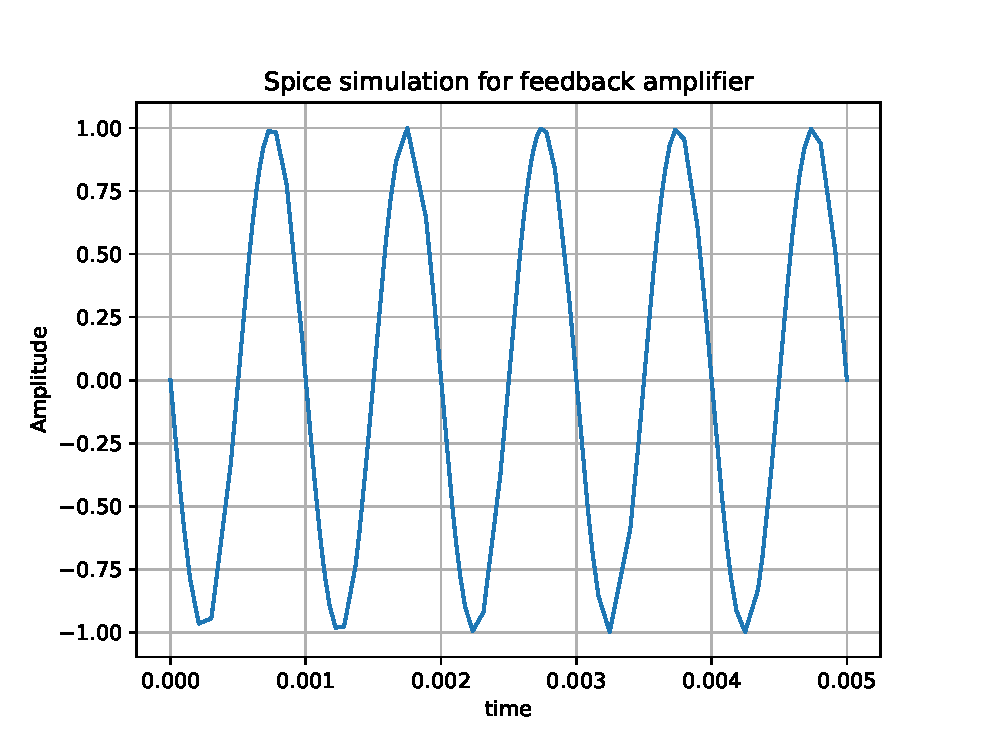
\includegraphics[width=\columnwidth]{figs/EE18BTECH11023/ee18btech11023_output.eps}
    \caption{output from feedback Amplifier}
    \label{fig:output}
\end{figure}
here we are using amplitude 1 for input signal. \\
then the output voltage will negative of the input signal. there will be no change in amplitude in output signal.\\

since the output and input are identically equal then there will be a minor change in output
\end{enumerate}

\subsection{Practical Case}
%\input{name}
%\input{./chapters/ee18btech11014_1.tex}
\end{document}

